%!TEX root = Main_Assignment3.tex
\documentclass[Main_Assignment3]{subfiles}

\begin{document}

\section{Specify a software architecture for the Alarm Clock}

The architecture of the system is created by dividing the system in small component, each testable with either a hardware component or with a software interface.
By layering the architecture, it is easier to increase cohesion and reduce the coupling, because each layer only sees layers beneith it and the software components only sees at the hardware it is responsible for.
This also creates an abstraction for the higher levels so they only see functions which handle tasks.

The design will be as in Figure \ref{fig:UML}.
To ensure the components can get the time and the alarm, a singleton is created to encapsulate the methods allowed to be called. 
It will allow \code{get}- and \code{set}-functions for both the alarm and the time. This way all classes have a single way of accessing the classes with anything regarding the time or the alarm.

Since both \code{Alarm} and \code{Clock} has the same key feature - showing a time (be it static or running) they inherit from the interface \code{Time}. 
This will ensure the same formating of the time for both \code{Clock} and \code{Alarm}.

The \code{Controller} containes the main loop and will check for all inputs.
It also creates all classes (except for the 2 \code{Time} classes created by the singleton \code{TimeHandler}). 
By doing this \code{Controller} can check whether the alarm should be triggered and activate the \code{Buzzer}, check inputs from \code{Buttons} to whether the current time or alarm should be changed, or the projector should be displaying the time.
If \code{Controller} can run a cycle at least every second, the alarm will go off within a second of the actual time.

The patterns to use are polymorphism with the interface and singleton to control the interface.

\begin{figure}[hbtp]
\centering
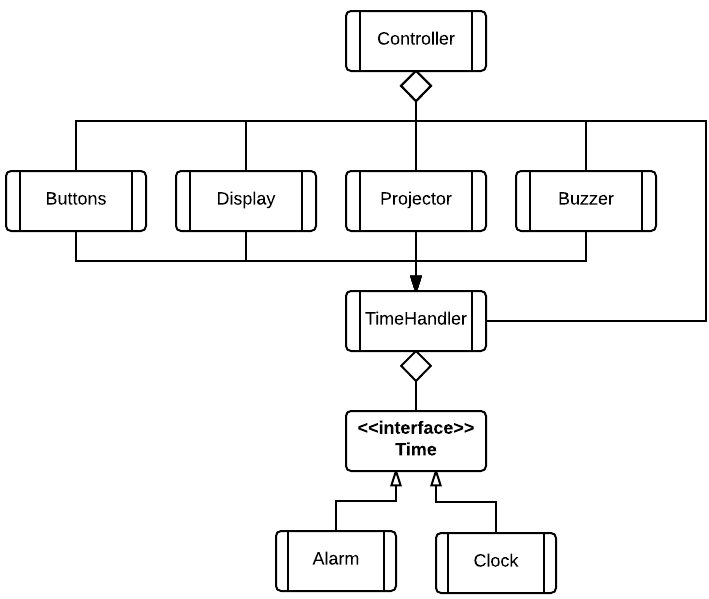
\includegraphics[width = 0.7\textwidth]{ArchitectureDiagram}
\caption{UML diagram}
\label{fig:UML}
\end{figure}

\end{document}